\documentclass[11pt,letterpaper]{article}

\usepackage{amsmath}
\usepackage{mathtools}
\usepackage{parskip}
\usepackage{siunitx}
\usepackage{enumitem}
\usepackage{calc}
\usepackage{tikz}
\usepackage{verbatim}

\usetikzlibrary{positioning}
\usetikzlibrary{arrows.meta}

\renewcommand\arraystretch{1.5}

\begin{document}
	\setlength{\parindent}{0pt}
	\setlength{\parskip}{1em}
	\title{Computing the Discretised Schr{\"o}dinger Equation}
	\author{Dr.\ D-Money}
	\maketitle
	\pagenumbering{arabic}

	\section{Math}
	\subsection{Nobody likes complex math libraries apparently}
	Start off with the Schr{\"o}dinger Equation in one-dimension:
	\begin{align*}
		i \hbar \frac{\partial}{\partial t} \psi &= \Big[-\frac{\hbar}{2m}\frac{\partial^2}{\partial x^2} + V(x)\Big] \psi
	\end{align*}
	Define the complex wave function $\psi$ in terms of its real and imaginary parts:
		\[\psi(x,t) = a(x,t)+ib(x,t)\]
		\[\psi =
		\begin{pmatrix}
			a(x,t) \\
			b(x,t)
		\end{pmatrix},
		i\psi = 
		\begin{pmatrix}
			-b(x,t)\\
			a(x,t)
		\end{pmatrix}\]
	Substituting this back into the Schr{\"o}dinger Equation, we see:
	\begin{align*}
		\frac{\partial}{\partial t} 
		\begin{pmatrix}
			-b(x,t)\\
			a(x,t)
		\end{pmatrix} &= 
		-\frac{\hbar}{2m}\frac{\partial^2}{\partial x^2}
		\begin{pmatrix}
			a(x,t)\\
			b(x,t)
		\end{pmatrix}
		+
		\begin{pmatrix}
			\frac{V(x)}{\hbar} a(x,t)\\
			\frac{V(x)}{\hbar} b(x,t)
		\end{pmatrix}
	\end{align*}
	\subsection{Discretising}
	Define the following variables:
	\begin{align*}
		i &= 0,\ldots,n\\
		x_i  &=  i\delta x\\
		\delta x &= \text{lattice spacing}\\
		\delta x &= \frac{L}{n}\\
		a(x_i,t) &= a_i(t)\\
		b(x_i,t) &= b_i(t)\\
		V(x_i) &= V_i
	\end{align*}
	Recall the second derivative approximation discussed in class:
	\begin{align*}
		\Big( \frac{\partial^2 a}{\partial x^2} \Big) x_i &\approx \frac{a_{i+1}+a_{i-1}-2a_i}{{(\delta x)}^2}\\
		\Big( \frac{\partial^2 b}{\partial x^2} \Big) x_i &\approx \frac{b_{i+1}+b_{i-1}-2b_i}{{(\delta x)}^2}
	\end{align*}
	We can see the following:
	\begin{align*}
		\begin{pmatrix}
			\partial_t (-b_i)\\
			\partial_t (a_i)
		\end{pmatrix}
		&=
		-\frac{\hbar}{2m \delta x^2}
		\begin{pmatrix}
			a_{i+1}+a_{i-1}-2a_i\\
			b_{i+1}+b_{i-1}-2b_i
		\end{pmatrix}
		+
		\begin{pmatrix}
			\frac{V_i}{\hbar} a_i(t)\\
			\frac{V_i}{\hbar} b_i(t)
		\end{pmatrix}
	\end{align*}
	\subsection{Removing dimensions}
	Define the following dimensionless quantities:
	\begin{align*}
		t&=\Big( \frac{2m\delta x^2}{\hbar} \Big) \tau\\
		&=(\delta t)\tau \leftarrow \text{dimensionless}\\
		V_i&=V_0 \widetilde{V}_i \leftarrow \text{dimensionless}
	\end{align*}
	Therefore:
	\begin{align*}
		\begin{pmatrix}
			-\frac{\partial}{\partial \tau} b_i(\tau) \\
			\frac{\partial}{\partial \tau} a_i(\tau)
		\end{pmatrix}
		&=
		\begin{pmatrix}
			2a_i-(a_{i+1}+a_{i-1}) \\
			2b_i-(b_{i+1}+b_{i-1})
		\end{pmatrix}
		+
		\begin{pmatrix}
			\frac{\delta t}{\hbar} V_i a_i(t)\\
			\frac{\delta t}{\hbar} V_i b_i(t)
		\end{pmatrix}\\
		\begin{pmatrix}
			\frac{\partial}{\partial \tau} b_i(\tau) \\
			\frac{\partial}{\partial \tau} a_i(\tau)
		\end{pmatrix}
		&=
		\begin{pmatrix}
			a_{i+1}+a_{i-1}-2a_i\\
			2b_i-(b_{i+1}+b_{i-1})
		\end{pmatrix}
		+
		\Big( \frac{\delta t}{\hbar} V_0 \Big)
		\begin{pmatrix}
			\widetilde{V}_i a_i(\tau) \\
			\widetilde{V}_i b_i(\tau)
		\end{pmatrix}\\
	\end{align*}
	Let us define $\beta$ such that:
	\begin{align*}
		\beta &\coloneqq \frac{\delta t V_0}{\hbar} \\
		&=\frac{2mL^2}{\hbar^3 n^2} V_0
	\end{align*}
	This is a dimensionless \textbf{coupling constant} on the \textbf{lattice}.
	\section{Computation}
	\subsection{Necessary resources/steps}
	\begin{description}[leftmargin=6em,style=nextline]
		\item[Next] Build an evolution scheme (algorithm) through \textbf{small} $(\delta \tau \ll 1)$ dimensionless time steps.
		\item[Tradeoff] We want to do evolutions through enough time steps to see disturbances in the wave function propogate across the entire length of the lattice. This means that if we step forward in time by $\delta \tau \approx 1$, we will need total time $N\delta t$, $N \approx \frac{L/\delta t}{\delta x / \delta t} = \frac{L}{\delta x} = n$.\par
	\end{description}
	If we choose $\Delta \tau \approx \frac{1}{m}$ ($m$ some integer $> 0$) we will need between $n \cdot m$ and \textbf{$2nm$ total time steps at a minimum} to see instructions that propogate across the total lattice.\\
	This means we prepare for 20,000 time steps on a 1000 point lattice (at the minimum) and probably more like 50,000 to 100,000.\par
	This means that if we want to see real results in a real time $T$, a single evolution time step must run in a time less than $10^{-5} T$. (e.g. If $T=10\si{\second}$ then a single evolution time step must run in $10^{-3}\si{\second}$)\par
	This gives you a rule of thumb about the time your code can take to do an evolution time step for data on the lattice. Clearly, to be fast you need to get single time step evolution execution time under a millisecond. Since this scales with the lattice size, you will probably want to debug a lot of code on lattices with smaller number of points (like 200 to 500).
	\subsection{Boundary conditions}
	Boundary conditions: $a_0=b_0=a_n=b_n=0$\par
	Hold these values fixed for ``box'' boundary conditions. These values are not \textbf{evolved} during the program run.
	\subsection{Going forward}
	\begin{description}[leftmargin=6em,style=nextline]
		\item[So far] We have translated a \textbf{partial differential equation} into a very large number of \textbf{ordinary differential equations} that are coupled together.
		\item[Next] We turn to the problem of approximating the time evolution in continuous time into an approximate series of time step evolutions. You will want to encapsulate the time evolution step in a single function or routine. I will suggest a baseline approach; however, there is room to upgrade or try out different evolution time step algorithms. Encapsulating this part of the program will facilitate experimentation.
	\end{description}
	\section{General Structure of Your Code}
	\begin{center}
		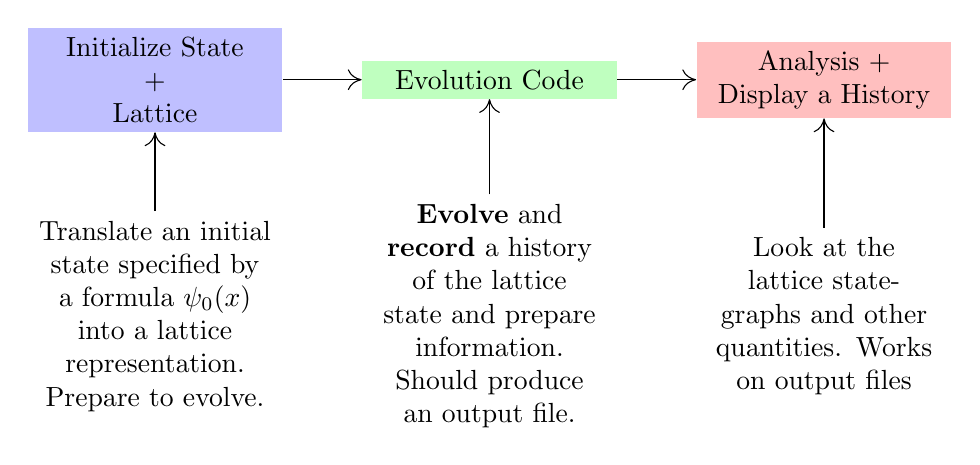
\begin{tikzpicture}
			\node[fill=blue!25, text width=3cm, align=center] (Initial) {Initialize State\\+\\Lattice};
			\node(Evolution)[fill=green!25, text width=3cm, align=center, right=of Initial]{Evolution Code};
			\node(Analysis)[fill=red!25, text width=3cm, align=center, right=of Evolution]{Analysis + Display a History};
			\node(Translate)[below = of Initial, text width=3cm, align=center]{Translate an initial state specified by a formula $\psi_0(x)$ into a lattice representation.\\Prepare to evolve.};
			\node(Evolve)[right = of Translate, text width=3cm, align=center]{\textbf{Evolve} and \textbf{record} a history of the lattice state and prepare information.\\Should produce an output file.};
			\node(Look)[right = of Evolve, text width=3cm, align=center]{Look at the lattice state-graphs and other quantities. Works on output files};
			\draw[-{>[scale=2.5,length=2,width=3]},line width=0.4pt] (Initial) to (Evolution);
			\draw[-{>[scale=2.5,length=2,width=3]},line width=0.4pt] (Evolution) to (Analysis);
			\draw[-{>[scale=2.5,length=2,width=3]},line width=0.4pt] (Translate) to (Initial);
			\draw[-{>[scale=2.5,length=2,width=3]},line width=0.4pt] (Evolve) to (Evolution);
			\draw[-{>[scale=2.5,length=2,width=3]},line width=0.4pt] (Look) to (Analysis);
		\end{tikzpicture}
	\end{center}
\end{document}
